\documentclass[journal,a4paper]{IEEEtran}
\usepackage{graphicx}
\usepackage[spanish]{babel}
\usepackage[utf8]{inputenc}
\usepackage{hyperref}

% para hacer figuras
%\begin{figure}
%    \centering
%    \includegraphics[width=3.0in]{myfigure}
%    \caption{Simulation Results}
%    \label{simulationfigure}
%\end{figure}
\newcommand{\tit}[1]{\textsc{\textbf{#1}}}
\begin{document}

\title{Navegación autónoma para robots móviles usando visión estéreo}
\author{Cintia Corti, Carlos Augusto Lyon Di Pietro, Facundo Pessacg, Kevin Allekotte}

\maketitle

\begin{abstract}
Como trabajo final de la materia \textsc{Visión en robótica} de \textsc{DC.UBA.AR}
presentamos un método para la navegación autónoma de robots usando visión estéreo.
La implementación se realizó para el \textsc{Exabot} usando las librerías \textsc{OpenCV} y \textsc{LibElas}.
\end{abstract}

\section{Introducción}
En este trabajo presentamos un método para la navegación autónoma de un robot basado en algoritmos de computer vision usando cámaras en estereo.

La visión en estéreo consiste de 2 cámaras alineadas en la misma dirección que toman las mismas imágenes desde puntos apartados ligeramente,
asemejandose al sistema de visión de los humanos y animales.
La idea es alinear las imagenes (previamente rectificadas) y calcular la disparidad en cada punto.
Cada punto del ambiente es captado por las 2 cámaras, y por propiedades trigonométricas vemos que la distancia del punto a las cámaras es proporcional a la diferencia de posicion horizontal observado entre las cámaras.
Así, un punto lejano va a proyectarse en las 2 imágenes en casi la misma posición, y un punto cercano a las cámaras va a proyectarse en posiciones distintas en cada cámara. 
Gracias a esta propiedad y calculando el mapa de disparidad entre las 2 imágenes podemos obtener una estimación muy buena de la geometría del espacio frente a las cámaras.
Un detalle no menor es que para calcular el mapa de disparidad de forma precisa las imágenes de las cámaras tienen que estar cuidadosamente rectificadas y alineadas. La rectificación corrige errores de deformación de las lentes para que las imágenes representen mas fielmente la proyección del espacio al plano de la cámara, y la alineación corrige la dirección en la que apuntan las cámaras para tener un sistema de referencia certero.

El objetivo del método es permitir a un robot la navegación autónoma, por lo que es importante la performance para poder correr en tiempo real y proveer acciones correspondientes basado en la visión. Vamos a usar las librerías de \texttt{OpenCV} para procesar los streams de video y \texttt{LibElas} para calcular el mapa de disparidad.

Para llevar a cabo una navegación autónoma se debe implementar una estrategia basada en la observación del mundo (cámaras, mapa de disparidad) que decida acciones a ser llevadas a cabo por los actuadores (ruedas del exabot).
Buscamos una estrategia que evite la colisión con objetos y avance hacia espacios libres del ambiente.

\section{Método}
\subsection{Calibración}
Las lentes de las cámaras tienen distorsiones que provocan que las imágenes captadas no representen exactamente la proyección de los objetos en el plano de captura. Por esto, y para obtener luego un mapa de disparidad preciso, es necesario aplicar las correcciones necesarias para ``rectificar'' las imágenes.

Para esto utilizamos software en el entorno \texttt{Matlab}, que permite calcular los parámetros intrínsecos y extrínsecos de las cámaras. Sacamos fotos estereoscopicas de una grilla -un damero- de dimensiones conocidas en distintas posiciones. Se indican características como origen y tamaño de la grilla, y el programa calcula las propiedades de la cámara como distancia focal, puntos principales, skew, dostorsión, rotación y distancia entre las cámaras.
Con estos parámetros podemos rectificar futuras capturas de la cámara para obtener imágenes alineadas y listas para procesar.

\begin{figure}[h!]
    \centering
    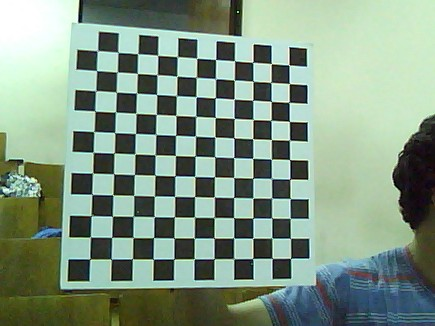
\includegraphics[width=0.8\linewidth]{calibracion1.jpg}
    
    \medskip
    
    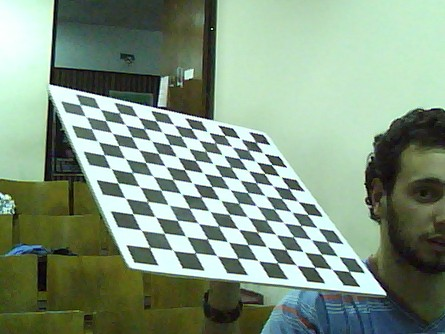
\includegraphics[width=0.8\linewidth]{calibracion2.jpg}
    \caption{Imagenes de prueba para calcular los parametros de rectificacion}
    \label{fig_calibracion}
\end{figure}

\subsection{Mapa de Disparidad}
Con las imágenes correctamente rectificadas podemos usarlas para calcular el mapa de disparidad.
Para esto vamos a usar la librería \texttt{LibElas} --Library for Efficient Large-scale Stereo Matching-- desarrollada por Andreas Geiger (Karlsruhe Institute of Technology).


\section{Propuesto}

\section{Experimentos}

\section{Conclusiones}

\section{Bibliografía}

\tit{LibElas}: Librería para computar mapas de disparidad a partir de pares de imagenes en escala de grises rectificadas. \url{http://www.cvlibs.net/software/libelas.html}

\bigskip

\tit{OpenCV}: Librería de funciones para computer vision en tiempo real. \url{http://opencv.willowgarage.com/}
\end{document}
